% small.tex
\documentclass{beamer}
\usetheme{Berlin}
\usecolortheme{beaver}
\usepackage[utf8]{inputenc}
\usepackage{graphicx}
\usepackage{mathtools}

\title[Verificatum]{El Gamal mixnät och\\ implementering av en verifierare}
\subtitle{Kandidatexamensarbete - SA104X - VT2013}
\author[Erik Larsson, Carl Svensson]{Erik Larsson \and Carl Svensson\\ \small{Handledare: Douglas Wikström}}
\institute{KTH, Skolan för datavetenskap och kommunikation}
\date{}

\begin{document}

\begin{frame}{Häftigt med riksdagsval}

\begin{itemize}
\item Rösta snabbt/säkert/hemligt
\item Verifierbart
\item Robust
\item Kanske ingen valvaka
\end{itemize}

\end{frame}
 A mix-net takes as input a list of encrypted messages. Verificatum is
 a reencryption mix-net. Such a mix-net consists of a number of
 servers, mix servers, which sequentially process the messages and
 reencrypts the list of messages and outputs them in a randomized
 order. After passing through all servers, the list of ciphertexts is
 decrypted and the result is the messages output in random order.

In the context of electronic voting a reencryption mix-nets may work
as follows.
\begin{enumerate}
\item The mix servers prepare the mix-net by generating public and
  secret keys.
\item Each voter encrypts his vote and appends it to a public list of
  encrypted votes.
\item In sequential order each mix server takes as input the list of
  encrypted votes, reencrypts and outputs them in a randomized order,
  replacing the previous list of encrypted votes.
\item After all mix servers have processed the list, each vote is
  jointly decrypted and posted on a bulletin board making the outcome
  of the election universally available without revealing how anyone
  voted.
\end{enumerate}

\begin{center}
  \makebox[\textwidth]{\includegraphics[width=0.7\textwidth]{../presentation/images/mix2.pdf}}
\end{center}


\section{Kryptografi}
\begin{frame}
\frametitle{Innehåll}
\tableofcontents[currentsection]
\end{frame}

\begin{frame}{Kryptografi}


\begin{columns}
    \begin{column}{0.45\textwidth}
        \begin{itemize}
			\item Historia
			\item Symmetrisk kryptering
			\begin{itemize}
				\item[-] Gemensam nyckel
			\end{itemize}
			\item Exempel
			\begin{itemize}
				\item[-] Caesar
				\item[-] Enigma
			\end{itemize}
		\end{itemize}
    \end{column}
	\begin{column}{0.55\textwidth}
    	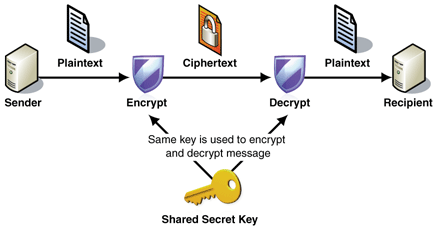
\includegraphics[width=\textwidth]{images/symmetric.png}
	\end{column}
\end{columns}

\end{frame}

\begin{frame}{Asymmetrisk kryptering}

\begin{columns}
    \begin{column}{0.45\textwidth}
        \begin{itemize}
			\item Räddningen
			\item Diffie \& Hellman
			\item Olika nycklar
			\item Okända parter kan kommunicera
		\end{itemize}
    \end{column}
	\begin{column}{0.55\textwidth}
    	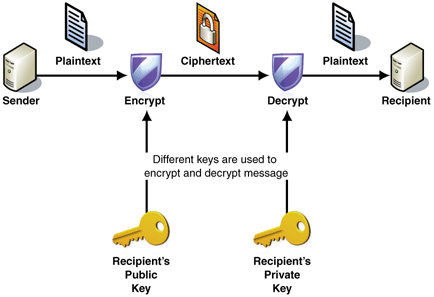
\includegraphics[width=\textwidth]{images/asymmetric.png}
	\end{column}
\end{columns}

\end{frame}

\begin{frame}{El Gamal-kryptografi}

\begin{columns}
	\begin{column}{0.5\textwidth}
		\begin{itemize}
			\item Givet y, g \& p, vad är x?
			\item Diskreta logaritmen svår
			\item Grunden i El Gamal-krypto
		\end{itemize}
	\end{column}
	\begin{column}{0.5\textwidth}
		{\LARGE $$y := g^x \mod{p}$$}
	\end{column}
\end{columns}

\vspace{3pt}

{\LARGE
\begin{align*}
y &\vcentcolon= g^{x} \,\,\,\,\,\,\,\,\,\, s\in \mathcal{R} \\
c &= (g^s, y^s\cdot m) = (u, v) \\
 m &= u^{-x}\cdot v
\end{align*}}

\end{frame}

\begin{frame}{Egenskaper hos El Gamal}

\begin{columns}
	\begin{column}{0.6\textwidth}
		\begin{itemize}
			\item Homomorft
			\begin{itemize}
				\item[-] Möjliggör flera lager kryptering
			\end{itemize}
			\item Generalisering till andra grupper
		\end{itemize}
	\end{column}
	\begin{column}{0.4\textwidth}
		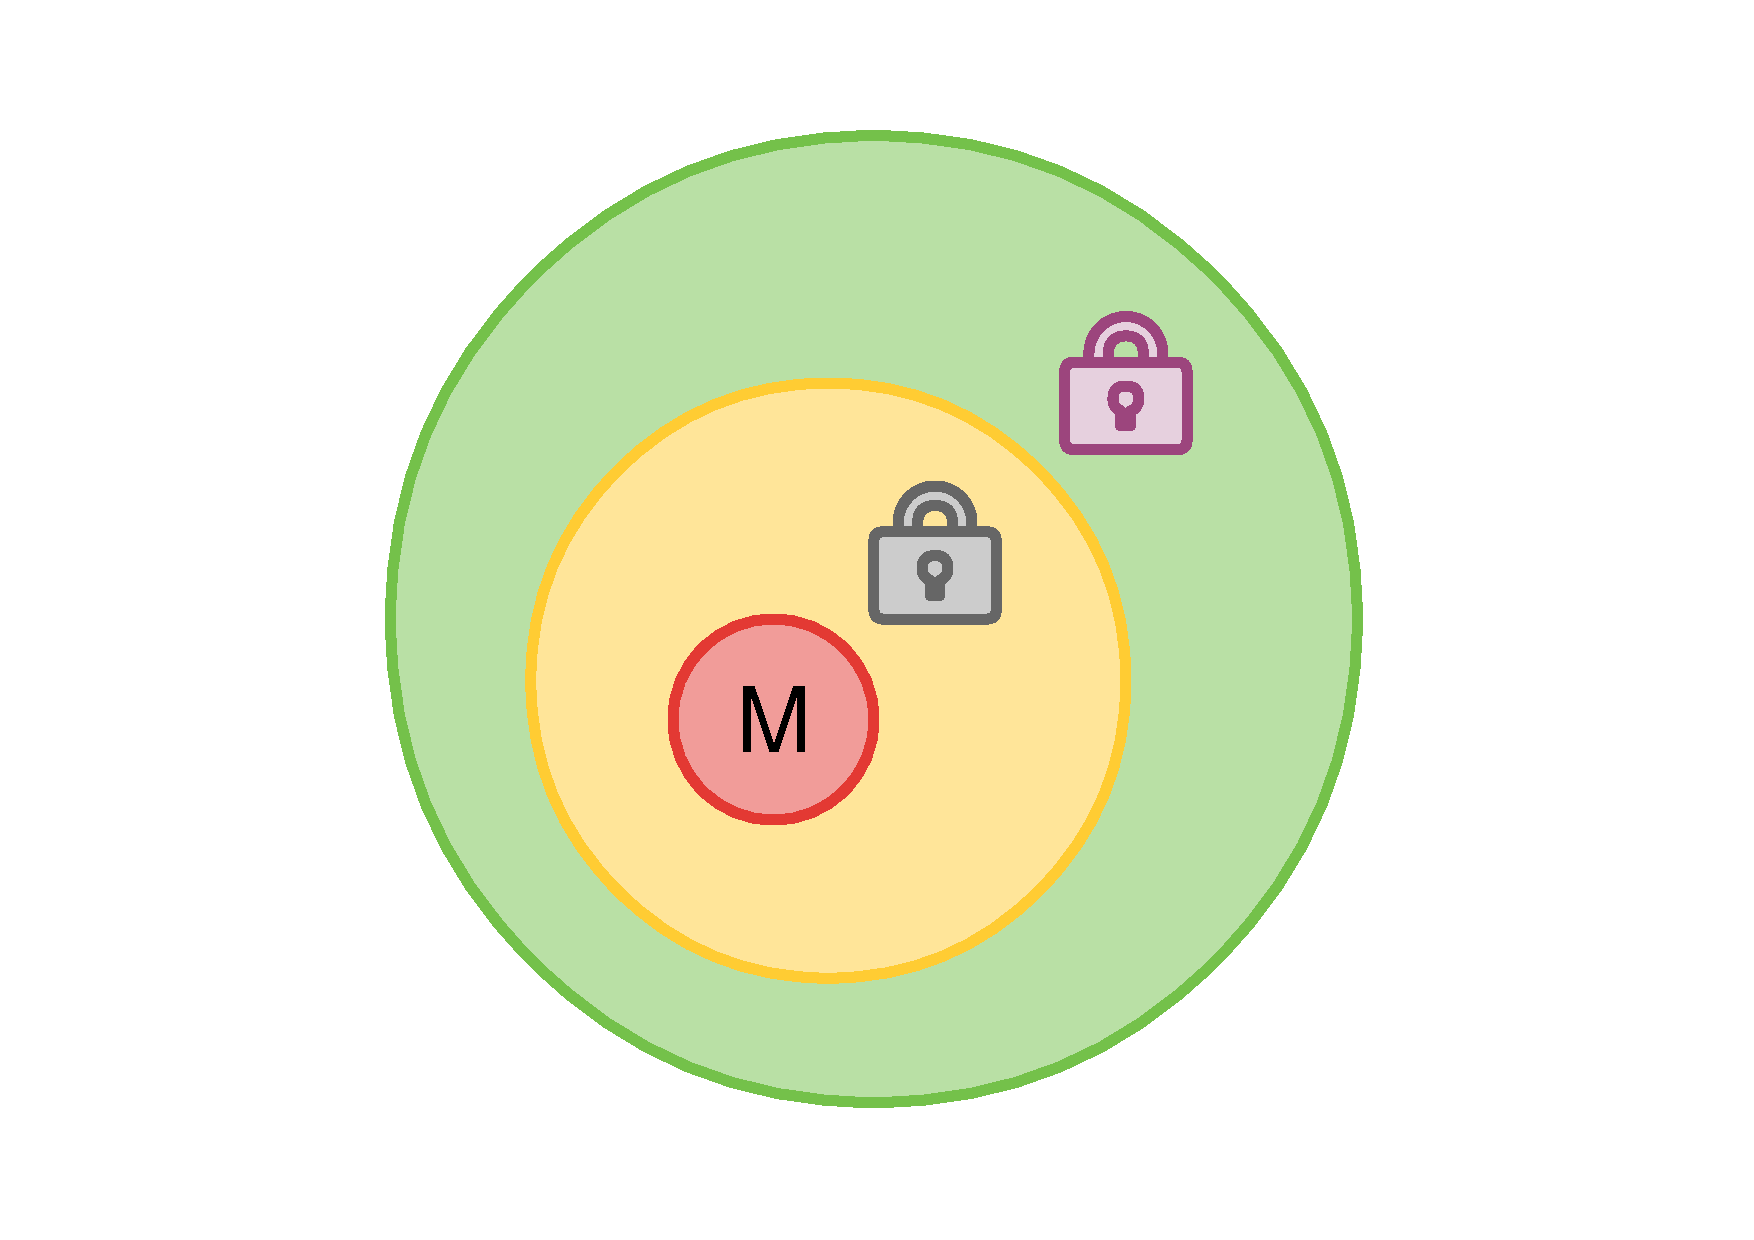
\includegraphics[width=\textwidth]{images/mix6.pdf}
	\end{column}
\end{columns}

\end{frame}

\begin{frame}{Zero-knowledge bevis}

\begin{itemize}
\item Bevis för ett påstende
\item Avslöjar inte något annat
\item Exempel
\begin{itemize}
	\item[-] Diskreta logaritmen
\end{itemize}
\end{itemize}

\end{frame}

\section{Mixnät}
\begin{frame}
\frametitle{Innehåll}
\tableofcontents[currentsection]
\end{frame}

\begin{frame}{Mixnät}

\begin{columns}
    \begin{column}{0.4\textwidth}
        \begin{itemize}
        	\item Mixnät blandar
        	\item Hur går detta till?
        \end{itemize}
    \end{column}
	\begin{column}{0.6\textwidth}
    	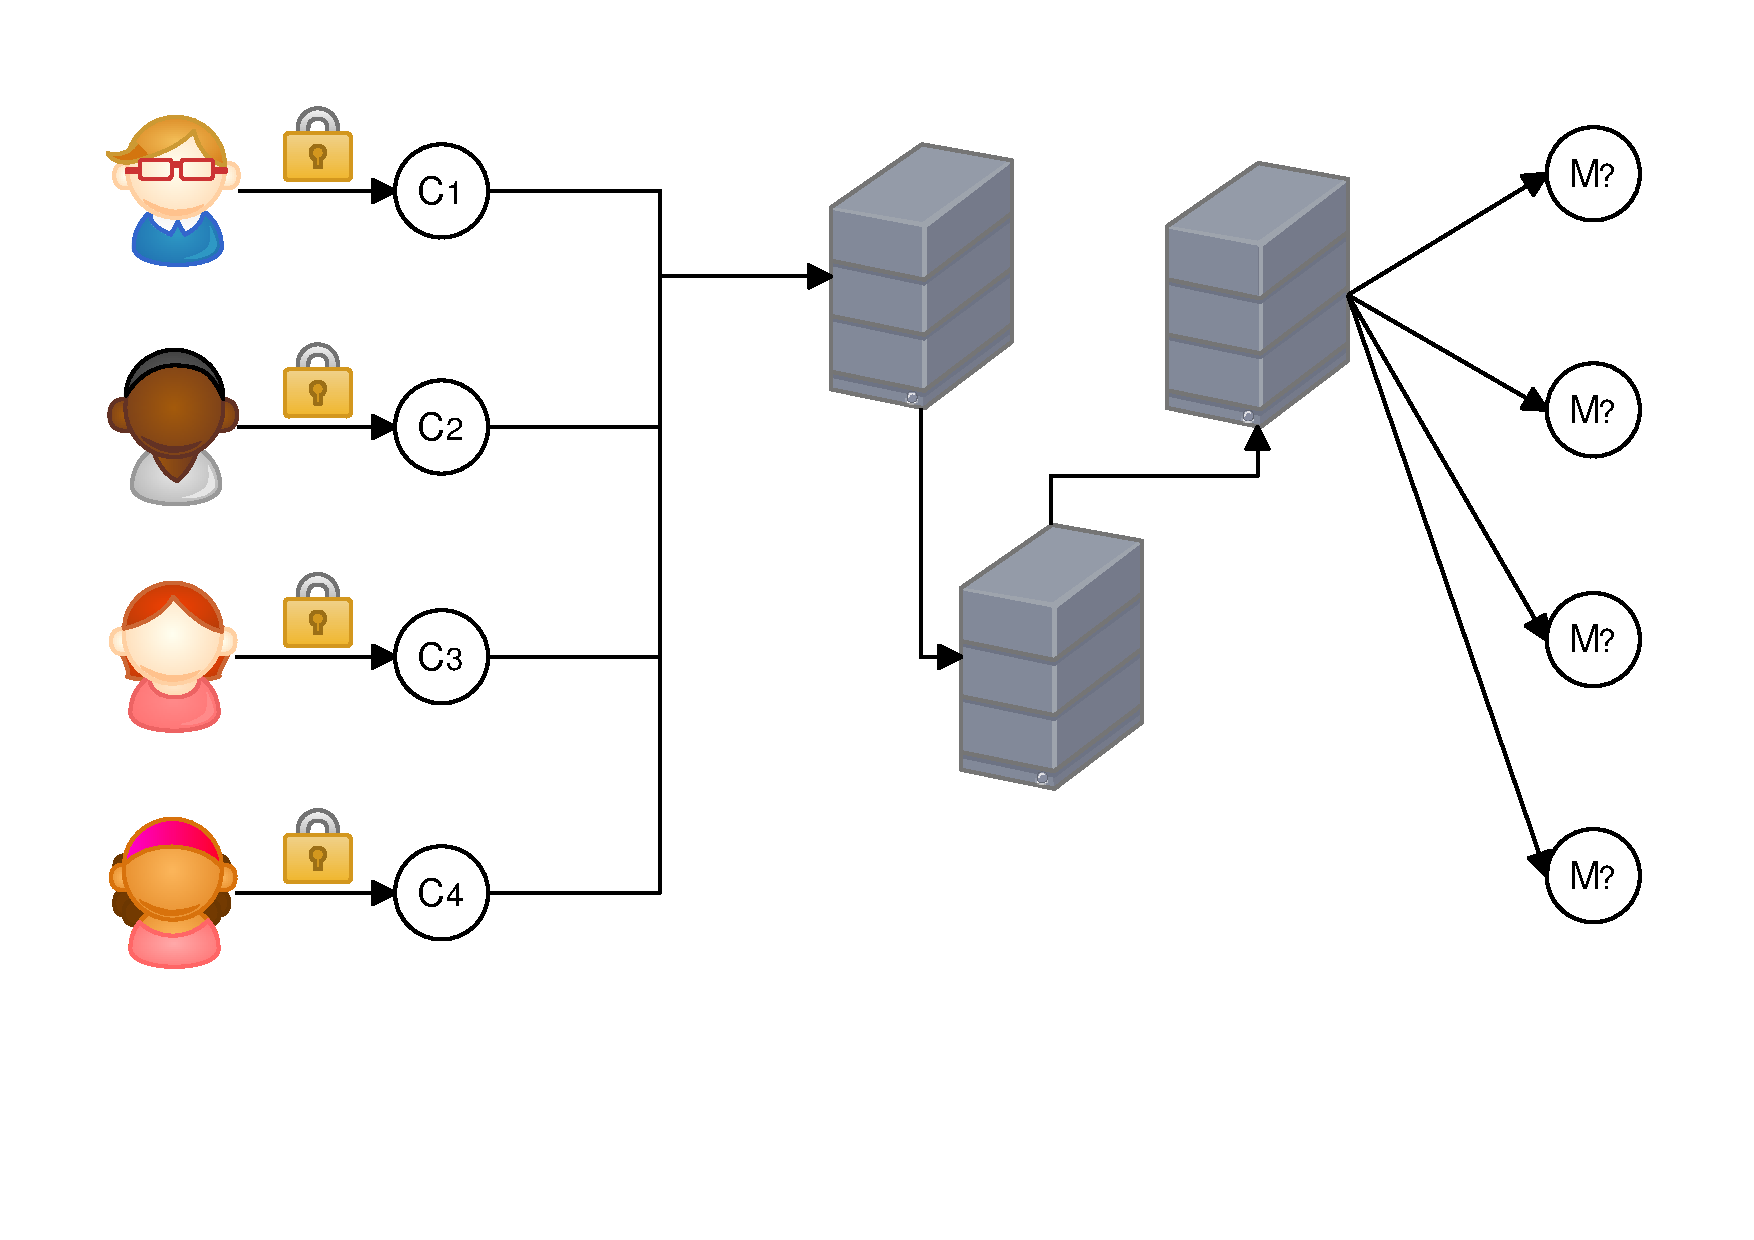
\includegraphics[width=\textwidth]{images/mix1.pdf}
	\end{column}
\end{columns}

\end{frame}

\begin{frame}{Hur fungerar varje server?}

\begin{columns}
    \begin{column}{0.4\textwidth}
        \begin{itemize}
        	\item Indata: kryptotexter
        	\item Kryptera om
        	\item Blanda
        	\item Mata ut
        \end{itemize}
    \end{column}
	\begin{column}{0.6\textwidth}
    	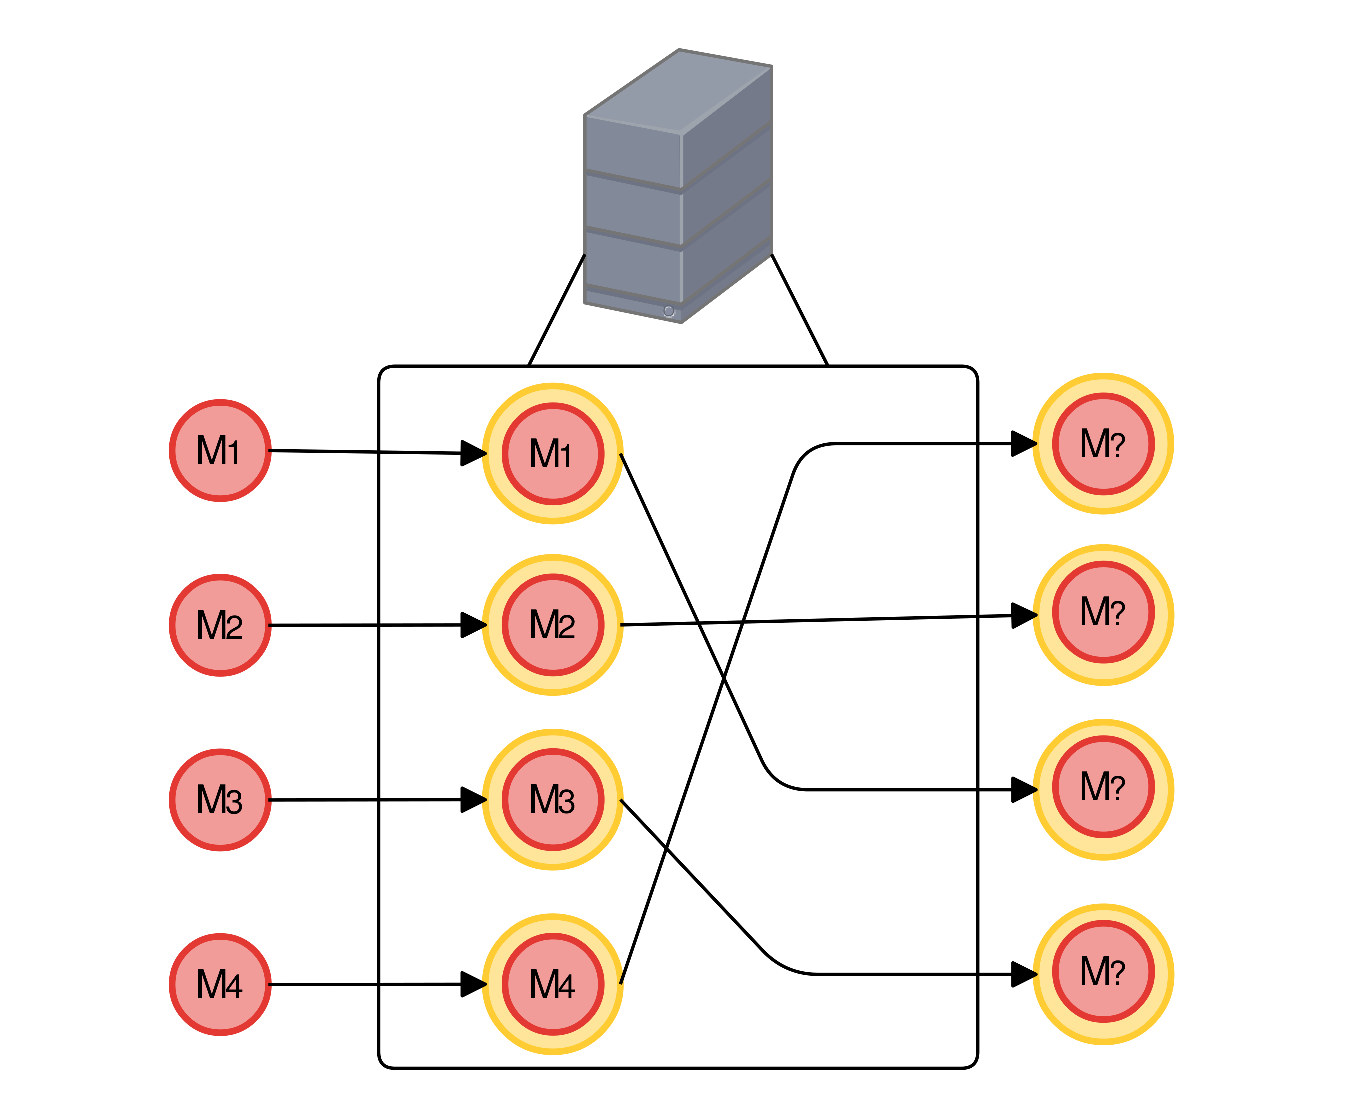
\includegraphics[width=\textwidth]{images/mix4.pdf}
	\end{column}
\end{columns}


\end{frame}

\begin{frame}{Hur kan vi verifiera att det blir rätt?}

\begin{columns}
    \begin{column}{0.4\textwidth}
        \begin{itemize}
        	\item Verifiering
        	\item Zero-knowledge
        	\item Extra data
        \end{itemize}
    \end{column}
	\begin{column}{0.6\textwidth}
    	\only<1>{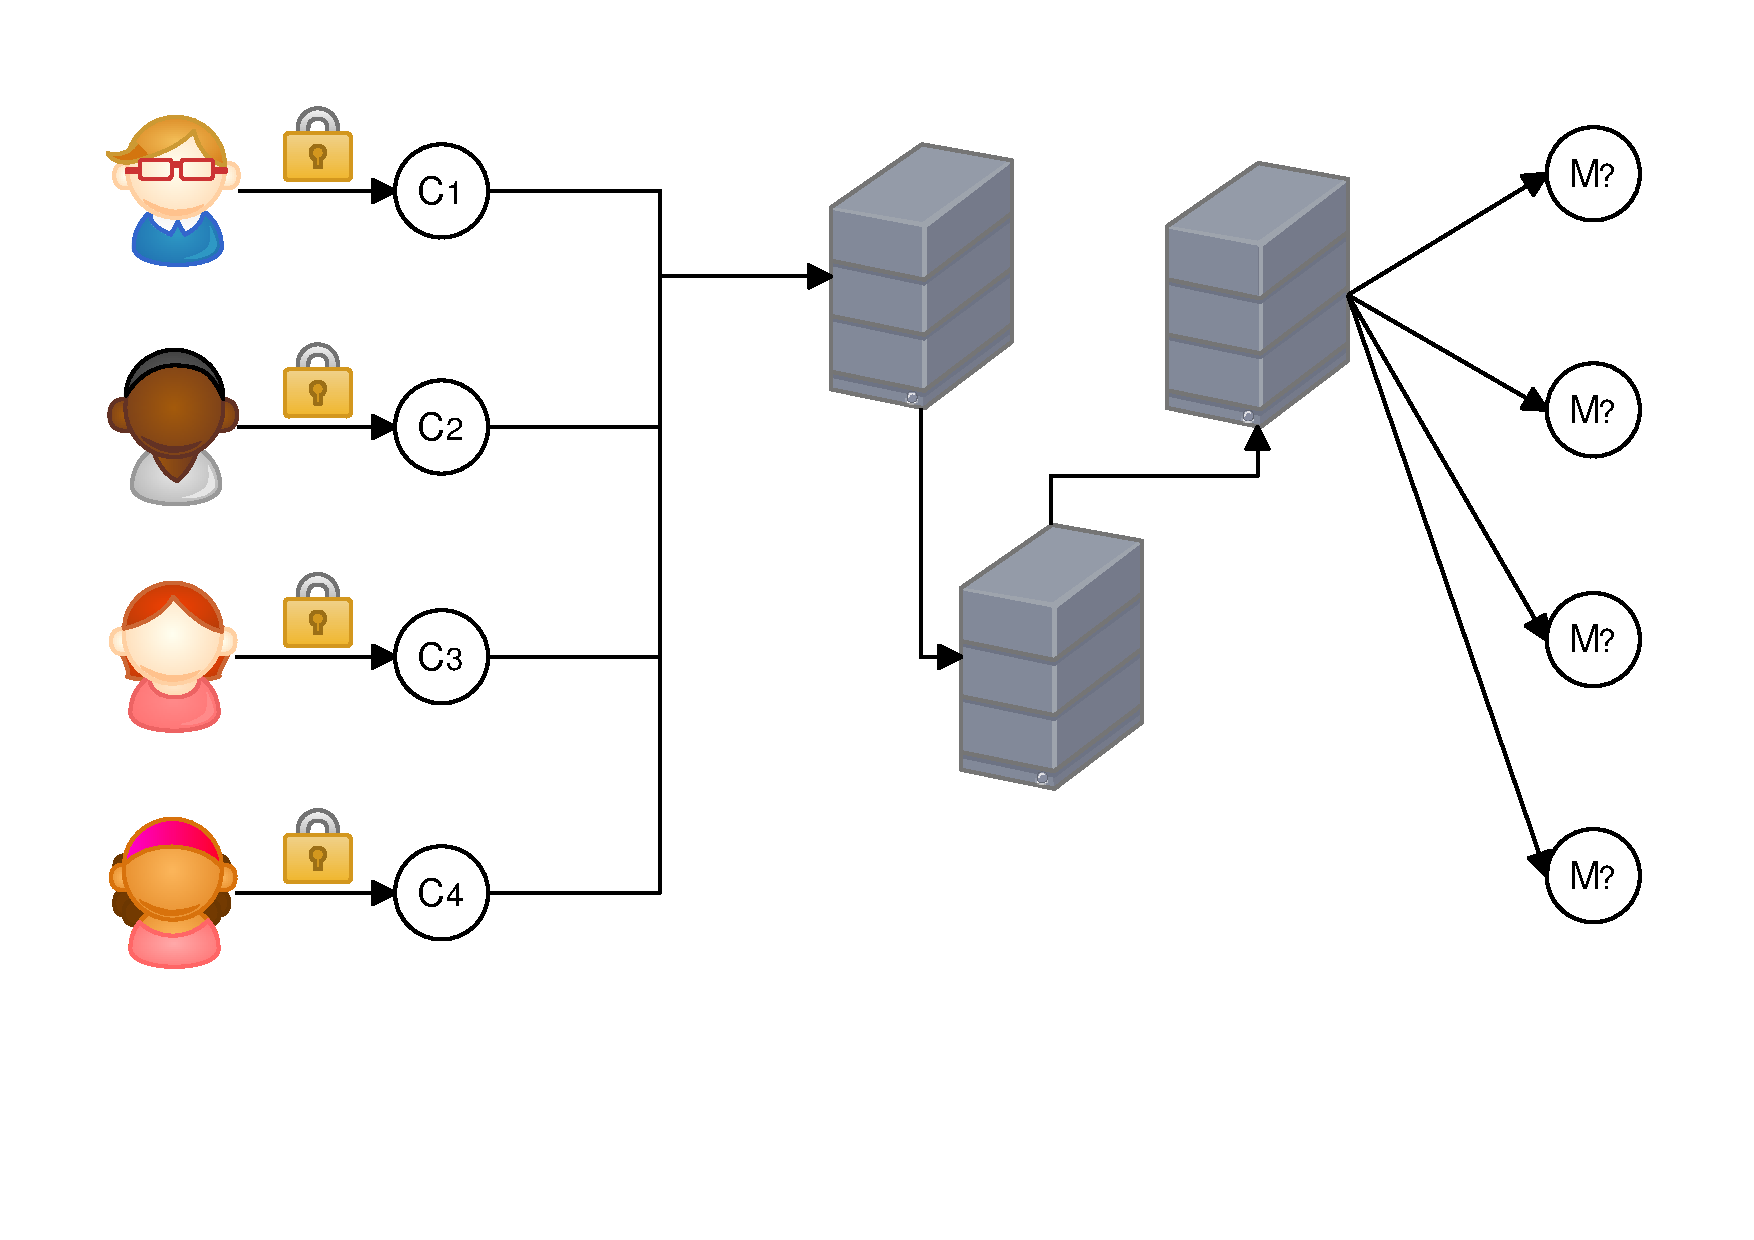
\includegraphics[width=\textwidth]{images/mix1.pdf}}
    	\only<2>{\includegraphics[width=\textwidth]{images/mix2.pdf}}
	\end{column}
\end{columns}

\end{frame}

\begin{frame}{Verifieraren analyserar körningen}

\begin{center}
  \makebox[\textwidth]{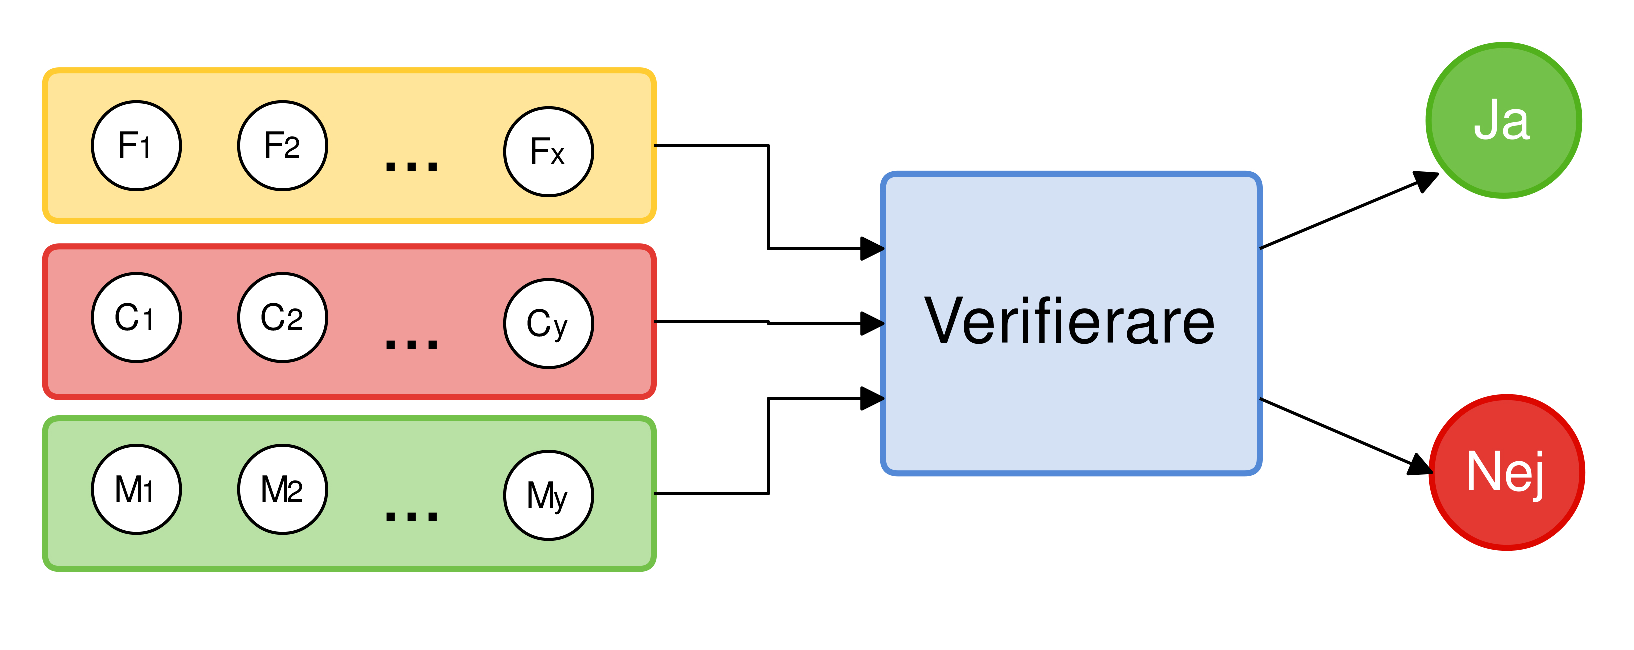
\includegraphics[width=\textwidth]{images/mix3.pdf}}
\end{center}

\begin{itemize}
\item Vi får reda på om allt gått rätt till
\item Inte möjligt att veta vilken röst som tillhör vem
\end{itemize}

\end{frame}

\section{Verificatum}
\begin{frame}
\frametitle{Innehåll}
\tableofcontents[currentsection]
\end{frame}

\begin{frame}{Vad är Verifactum?}

\begin{itemize}
\item Implementation av mixnät
\item Verifierbart
\item Vem som helst ska kunna verifiera
\item Specifikationsdokument
\begin{itemize}
	\item[-] Är det korrekt?
	\item[-] Är det användbart?
\end{itemize}
\end{itemize}

\end{frame}

\section{Implementation of a Verifier}

\subsection{Verificatum Mix Network (TODO)}

Verificatum is a reencryption mix-net based on the El Gamal
cryptosystem \cite[p.~1]{wikstrom1}. During execution it generates a
verifiable proof of correctness. 


Verificatum has different types of execution, all of which require
different verification. There is mixing, shuffling + combination?

There is a key distribution phase.

There is a shuffling phase, during which each server provides a proof
of shuffle (Beskriv vad detta är)

\subsection{Specification}

The document \cite{wikstrom1} describing a verifier for correct execution of the
Verificatum mix-net contains detailed instruction for the
implementation. A number of subtasks are described, some of which may
be implemented independently. The subtasks include include
implementation of general representation of data, an arithmetic
library needed to perform group operations, the cryptographic
primitives and the structure of files created during an execution of
the mixnet. Furthermore, all algorithms executed during the
verification are described in detail in order to allow an independent
verifier.

\subsection{General Design Choices}

The first implementation choice was which programming language to
use. We wanted to use well established technologies and have a good
performance [REF] on the verifier. Considering these criteria and our
programming skills, the choice was made between C, C++ and Java. Since
other groups are working on implementations in Java we decided to use
C or C++ and since we wanted to use features such as operator
overloading and some OOP, we settled on C++.

The program consist of a few different parts. To represent the various
mathematical objects in the calculations, we created a collection of
classes of function called a \emph{byte tree}. These store group
elements and a few other types of data as specified in the
specification.

We wanted to keep the verifier as close to the specification in layout
as possible. Apart from some cryptographic primitives and the byte
trees, there is almost no code repetition in the verifier. This meant
that we would gain little to nothing by designing any kind of class
structure or abstractions.

The byte trees were modelled with a few classes representing nodes and
leaves. This enabled us to hide away complex operations behind simple
interfaces which resulted in a more readable and maintainable code
throughout the rest of the verifier.

\subsection{Tools}

We developed the program on two different platforms. The code was kept
in a git repository and hosted on GitHub. One of the development
platforms used OS X 10.8 with Emacs and g++ 4.7. The other used
Windows 8 with Visual Studio 2012. We generated reference documents
for the program with Doxygen.

\subsection{Third Party Libraries}

The verifier makes use of a few third party libraries. The actual
arithmetic in the byte tree nodes are done with the GMP arithmetic
library. This enables us to handle arbitrary large numbers which are
used in cryptography. We also use RapidXML for parsing the
protInfo.xml file at the very beginning of the verifier. For
cryptographic hash functions we use OpenSSL and finally for unit
testing we use Google's Google Test library.

\subsubsection{Arithmetic Library}

For the actual arithmetic done in the IntLeaf node class we use the
GNU Multi-Precision Library (GMP). On Windows this is replaced by the
library Multiple Precision Integers and Rationals (MPIR), a drop in
replacement which is easier to compile on windows systems. We chose
GMP because it is a well known, very stable and free library for
bignum operations.

\subsubsection{XML Parser}

RapidXML is used to parse the protInfo.xml file in the beginning of
the algorithm. Since this is a very simple operation and we only do
this once, we wanted a lightweight library to do the XML
parsing. RapidXML consists of a few header files and has an easy to
use interface.

\subsubsection{Cryptographic Primitives}

All of the PRGs and ROs in the verifier are implemented in the
verifier but at the core they all depend on cryptographic hash
functions such as the SHA-2 family. We take these functions from the
OpenSSL library. OpenSSL is a well known, stable and free library for
various cryptographic related functions.

\subsubsection{Testing}

To test the byte tree classes and our cryptographic functions we used
some unit testing. We used Google Test as our unit test framework
because it was simple and easy to use. The unit tests were invaluable
in tracking down subtle bugs in our byte tree implementation,
especially regarding memory management.

\subsection{Math Library - The Byte Tree}

To facilitate for the various calculation that needs to be done with
various mathematical objects. We created a collection of \emph{byte
  tree} classes. The classes use the GMP library internally to perform
the actual arithmetic calculations. The classes then wrap these
operations in a class hierarchy which enables us to create arrays and
trees and perform calculations with these compound structures. There
are also functions to import strings and files and convert them into
these classes. The classes can also be serialized into arrays and
strings which are used for testing and debugging purposes.

\subsection{Pseudorandom Generators and Random Oracles}

The specification also provide details on the PRG:s and RO:s used in
Verificatum. These primitives are implemented as classes which are
instantiated to perform their respective operations as described
earlier. These classes use hash functions from the OpenSSL library
internally to perform the hashing part.

\subsection{Verifier}

To keep track of some data which is persistent throughout the
execution, we created a structure to hold this data. This structure
was created at the beginning of the execution and then passed around
to the different algorithms.

Apart from the byte tree classes and the cryptographic primitives, we
needed a few helper functions. The purpose of these functions was to
check that some different byte tree adhered to a certain structure.

Each named algorithm in the specification was implemented as its own
function. The functions became long but since none of the code is
repeated and the possibilities for isolated testing was minimal, we
chose to not split up the algorithms into several functions.

\subsection{Testing and Debugging}

For the \emph{byte tree}, PRG and RO classes, a small collection of
unit tests were created. The tests for the PRG and RO classes were
taken from the test vectors chapter in the specification while the
byte tree tests were created by us. The tests were implemented with
the Google Test test framework.

When all the parts of the program had been implemented we received
test data from Wikström to verify that the program worked. The data
contained two small instance with all the input files required by a
normal run of the verifier. Additionally the test data contained the
correct state of key variables throughout important steps of the
execution. The debugging was done in Visual Studio. By stepping
through the program and comparing states against the test data we
removed bugs in the program.

Fungerade sen?

\section{Results}

\subsection{Resulting Code}

Our resulting implementation of the mix-net consists of about 5500 lines of C++ code divided into three parts, Arithmetic, Crypto and Verifier. The first two parts are the byte tree classes and the cryptographic primitives respectively. The verifier part contains the actual verification algorithms.

The code is available on GitHub\cite{github} but should not be considered a stable release.


\subsection{Comments on the Documentation}

The overall impression of the documentation was that it contained all
information needed to implement the verifier. There were, however,
errors affecting the execution of the verifier. Some of the problems arising from these
errors were overcome after discussion with Wikström. See Appendix B
for a complete list with errors found and specific comments about the
report.

In the absolute beginning of the document, the reader is thrown into
details about the zero-knowledge proofs used in VMN. A more gentle
approach would be to introduce the VMN without assuming too much
acquaintance with it or provide the means for the reader to do so on
his or her own. It would also be appreciated if the document contained
a description of Pedersen commitments.

The background, including a description of a mix-net based on the El
Gamal cryptosystem, is clear and concise. After the background, the
document contains a list of manageable subtasks in order to facilitate
implementation. This list was appreciated as it gave someone
unacquainted with Verificatum ideas of suitable starting points.

Chapters 4 through 6 contain necessary and easily accessible
information. However, chapter 4 on byte trees and chapter 6 on
representation of arithmetic objects are closely related and could
advantageously be presented together while bringing up the
cryptographic primitives of chapter 5 afterwards. The part on deriving
group elements from random strings depends on chapter 5 and
consequently needs to be presented after. See Appendix C for a
clarification on these comments.

Chapter 6.6 on Marshalling Groups contains specific details regarding
the Verificatum software with strong connections to Java. This chapter
could be rephrased to only include information actually needed for
implementation of a verifier.

Lastly, the chapter on verification of Fiat-Shamir proofs relies
heavily on the derivation of group elements from random strings. By
moving chapter 7 to before the chapter on cryptographic primitives,
usage of the document will probably demand less page turns.

\subsection{Conclusion}

Regarding the programming it would have helped with having more layers
of abstractions in the code. Specifically, some classes representing
various mathematical objects, such as group elements, would have made
the code easier to maintain. We believe that a more solid
understanding of the structure of VMN before we started programming
would have helped in creating a better structure of the verifier. The
choices of third party libraries were good and they were all easy to
use in our project. This also makes the amount of code which need to
be written smaller. The lack of test data greatly increased the difficulty of implementing the verifier.

The specification document for the verifier does include all the
information required to write the verifier. However, the structure
could be improved for greater readability. There is also some
unnecessary information in the document. Lastly, the document could
benefit from an improved description of the VMN so that one easier can
get a better understanding of what approach to take when implementing
the verifier.
\section{Avslut}
\begin{frame}
\frametitle{Innehåll}
\tableofcontents[currentsection]
\end{frame}

\begin{frame}{Vad innebär allt detta?}



\begin{columns}
    \begin{column}{0.6\textwidth}
        \begin{itemize}
			\item Elektronisk röstning är möjligt
			\item Inte riktigt där \emph{än}
			\item Verificatum i norska valet
		\end{itemize}
    \end{column}
	\begin{column}{0.4\textwidth}
    	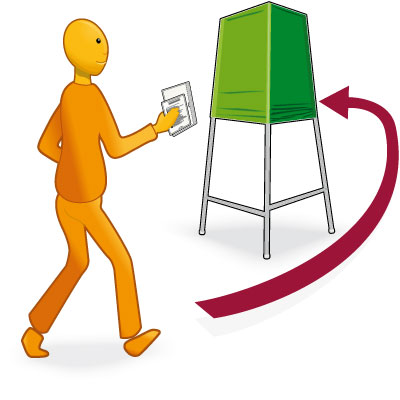
\includegraphics[width=\textwidth]{images/rosta.jpg}
	\end{column}
\end{columns}

\end{frame}

\begin{frame}{Tack för oss! Frågor?}

\begin{columns}
    \begin{column}{0.4\textwidth}
        \begin{itemize}
			\item Tack för att ni lyssnade!
			\item Har ni frågor?
		\end{itemize}
    \end{column}
	\begin{column}{0.6\textwidth}
    	\includegraphics[height=0.7\textheight]{images/interrobang.png}
	\end{column}
\end{columns}

\end{frame}

\end{document}
